\section{Architectural Design}

\subsection{High level components and interactions}
The following block diagram describes the overall solution design by giving an high-level perspective of all main application roles. In particular, it makes easy to understand the partition of software service components across the solution realm and their interaction mechanisms through internal subsystems interfaces.

\begin{figure} [h!]
\centering
\includegraphics[scale=0.66]{{Figures/Architecture.png}}
\label{fig:Architecture}
\end{figure}

% \begin{wrapfigure}{r}{5.5cm}
% \caption{A wrapped figure going nicely inside the  text.}\label{wrap-fig:1}
% \includegraphics[width=5.5cm]{Figures/Architecture.png}
% \end{wrapfigure} 
%------------------------------------------
% {\lipsum[2-3]
% \par
% Figure~\ref{wrap-fig:1} is a wrapped figure.}


\begin{itemize}
\item{\textbf{Client side applications}}\newline
Represent the pool of user interactive applications made of both mobile applications running on user owned devices and onboard ride assistants running on the onboard infotainment devices of PowerEnJoy Cars.
\item{\textbf{Vehicle management platforms}}\newline
Represent the pool of embedded controllers devoted to remotely interfacing the vehicle hardware.

\item{\textbf{Front-end service roles}}
\begin{itemize}
\item{\textbf{Client Worker}}\newline
A single Client Worker node acts as a proxy between any remote interactive client and back-end components. In other words, it exposes all interfaces needed by any application the end user directly interacts with to allow decoupling from core service feature components, avoiding any client technology-dependent issue to be addressed by back-end design decisions. It is able to validate an existing authentication token avoiding redundant messaging to the back-end. It also provides access to static/cached resources and it's designed to be fully stateless, allowing automatic/on-demand scale-up of nodes instances to distribute workload across, dramatically increasing reliability and performance. A CW node can return execution results to remote clients both in synchronous (request/response) or asynchronous mode (event/notification).
\item{\textbf{Vehicle Worker}}\newline
A single Vehicle Worker node acts as a proxy between any remote supported vehicle platform and back-end components. In other words, it exposes all interfaces needed by any supported vehicle to allow decoupling from core service feature components, avoiding any platform-dependent issue to be addressed by back-end design decisions. it's designed to manage and keep track of an huge number of status/telemetry updates. Inside a VW node, updates from multiple different vehicles are stored until expiration and timestamped. When an event is triggered by a new vehicle the node registers itself to the back-end as the handler of that vehicle. This way we are still allowing automatic/on-demand scale-up of nodes instances to distribute workload across, dramatically increasing reliability and performance. A VW node works only in asynchronous mode (event/notification) w.r.t. the remote vehicle.
\item{\textbf{Elastic load balancing request router}}\newline
Available from any common cloud provider. Provides automatic scale-uo/-down of nodes instances based on their resources utilization and redirects request messages to nodes guaranteeing a fair workload distribution across them.
\item{\textbf{Elastic load balancing event hub}}\newline
Available from any common cloud provider. Provides automatic scale-uo/-down of nodes instances based on their resources utilization and manages to forward an huge number of event messages to nodes guaranteeing a fair workload distribution across them.
\item{\textbf{Elastic async push messages dispatcher}}\newline
Available from any common cloud provider. Provides efficient queuing of large number of messages to dispatch to multiple groups of targets. It also takes care of creating and keeping up network notification channels.
\end{itemize}

\item{\textbf{Back-end service roles}}
\begin{itemize}
\item{\textbf{Service Back-end Logic Worker}}\newline
Each SBL Worker node provides all PowerEnJoy core service features. They actually runs the whole service logic decoupled from any presentation layers and communication protocols to front-end devices. Each SBL Worker is fully stateless and supports simultaneous multiple worker's instances with obvious redundancy and performance advantages. For better performances a single node is restricted by design to only serve a specific service zone. An SBL Worker also provides some data access optimization (i.e. caching, mirroring) to inner components and can be instantiated both automatically by scaling managers or manually if needed. For example, if interface compatibility is preserved, will be possible to manually instantiate an SBL Worker running a different software version, allowing seamless on-field testing, debugging and upgrade experience.
\item{\textbf{Elastic load balancing service bus}}\newline
Available from any major cloud provider. Allows efficient interconnection of components between back-end and front-end roles. It can be configured to act as an automatic scaling manager if the cloud provider offers that option.
\item{\textbf{User Account Data}}\newline
Stores all account related data such as user credentials, personal identity, driving license, credit card details and payments history. Accounts are unique and shared across all PowerEnJoy covered zones.
\item{\textbf{Configuration Data}}\newline
Stores all service global parameters that system administrators can modify according to their needing, like those related to discounts and penalties policies, service fares, booking timeouts and so on.
\item{\textbf{Single Zone Data}}\newline
Stores all data related to a single zone covered by the PowerEnJoy service such as vehicles, Safe and Special Parking Areas, active bookings and any parameter override that should only be applied to that zone.
\item{\textbf{Management API}}\newline
Provides administrative and monitoring low-level access to core components, designed to be easily interfaced with any business management platform (ERP, CRM, enterprise portals etc.). It's existence has been taken into account only to adapt current solution design for future software evolution. No further design or development effort will be spent on this component unless requirements renegotiation. As of this document revision, the described solution is fully functional and serviceable without this component by direct manipulation of data.
\end{itemize}
\end{itemize}

\subsection{Component view}
This section contains the component view and the descriptions of each component. Their interfaces are described in the section 2.5 Component interfaces.
\subsubsection{Service Back-end Logic}
\begin{figure} [h!]
\centering
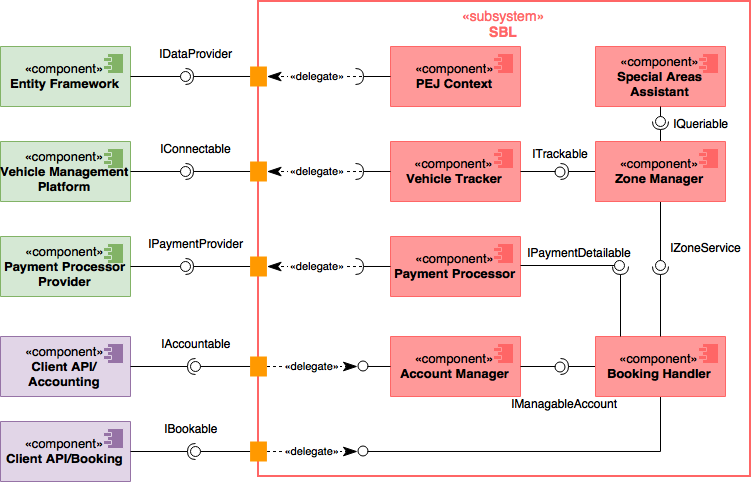
\includegraphics[scale=0.5]{{Figures/Component_Diagram/SBL.png}}
\label{fig:SBL}
\end{figure}
The Service Back-end Logic subsystem is composed of:
\begin{itemize}
    \item\textbf{PEJ Context}\newline
    It is the component through which all the others can access data entities containing all the information and details about zone, vehicles, accounts and configurations.
    \item\textbf{Zone Manager}\newline
    It is the component that connects Booking Handler to related Vehicle Tracker and Special Parking Areas of inherent zone applying any zone-specific configurations.
    \item\textbf{Special Areas Assistant}\newline
    It is the component that provides the set of functions needed to get lists of Special Parking Areas satisfying specific requirements.
    \item\textbf{Vehicle Tracker}\newline
    It is the component that asynchronously interacts with the Vehicle Management Platform collecting data required by other components.
    \item\textbf{Booking Handler}\newline
    It is the component that manages the bookings and their related rides. It provides the functions for creating a new booking, having it progress to a ride and ending it creating a pending payment record of appropriate amount.
    \item\textbf{Payment Processor}\newline
    It is the component in charge of managing pending payments issuing requests to Payment Processor Provider.
    \item\textbf{Account Manager}\newline
    It is the component in charge of managing user data when he creates a new account, signs in, asks for his personal profile page or wants to modify personal details.
\end{itemize}
and it interacts with:
\begin{itemize}
    \item\textbf{Entity Framework}\newline
    It is the set of external sub-components that is in charge of binding data entity models to corresponding datasource schema.
    \item\textbf{Vehicle Management Platform}\newline
    It is the component that connects to a vehicle in order to get its data including positions, battery level, engine ignited, and all the other data provided by the vehicle sensors.
    \item\textbf{Payment Processor Provider}\newline
    It is the third party system PowerEnJoy relies on in order to bill the customer's credit cards.
    \item\textbf{Client API/Accounting}\newline
    It is the middleware between SBL and mobile apps the user interact with. It exposes only the set of interfaces required to register, sign in or modify the personal user data.
    \item\textbf{Client API/Booking}\newline
    It is the middleware between SBL and mobile apps the user interact with. It exposes the set of interfaces required to create or cancel a reservation, and manage the whole ride including access to the map of available vehicles, the position of the reserved Car or to get lists of Special Parking Areas.
\end{itemize}
%Add \newpage here if necessary
\newpage

\subsubsection{Mobile App}
\begin{figure} [h!]
\centering
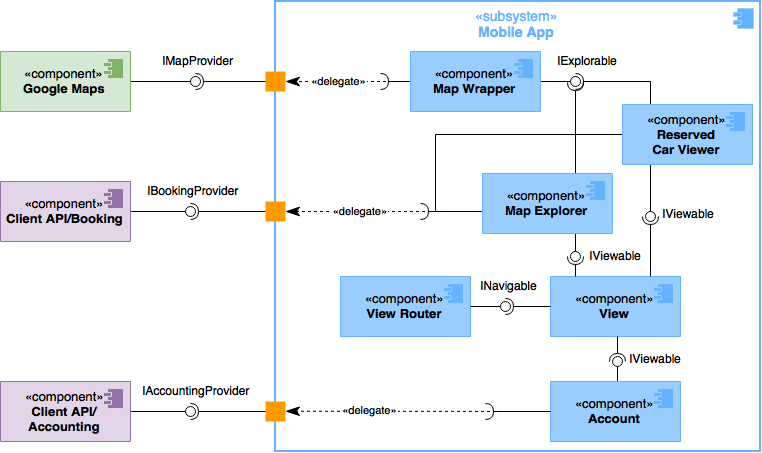
\includegraphics[scale=0.5]{{Figures/Component_Diagram/MobileApp.png}}
\label{fig:MobileApp}
\end{figure}
The Mobile App is composed of:
\begin{itemize}
    \item\textbf{View}\newline
    It is a set of sub-components representing something the user can see and interact with; each sub-component renders the view relying on the view models provided by other components and translates user inputs to well-formed and sanitized requests sent through other components.
    For this application this set includes sub-components related to map, sign-in and sign-up forms, account and reservation management.
    \item\textbf{View Router}\newline
    It is the component that implements and keep tracks of navigation paths across various views, providing for a given view model the right view component to be navigated that is able to present it to the user. It also implements backward navigation feature.
    \item\textbf{Map Wrapper}\newline
    It is the component that wrap the outsourced map images into an user control that makes them scrollable and zoomable, with the ability to overlay custom objects in defined position. It allows the application not to be coupled to a specific third-party maps provider.
    \item\textbf{Map Explorer}\newline
    It is the component that takes the map provided by the Map Wrapper and takes care of showing the position of all available Cars. These positions are obtained via Client API/Booking call.
    \item\textbf{Reserved Car Viewer}\newline
    It is the component that takes the map provided by the Map Wrapper and adds the position of the reserved Car. This position is stored within the app or it is requested via Client API/Booking call if necessary. It allows the user to request a booking cancellation or the unlock of its associated Car.
    \item\textbf{Account}\newline
    It is the component in charge of all the account-related functions. After the sign in, it provides the view with the user avatar, so that it can be used as access to the user personal data page which is also managed by this component.
\end{itemize}
and it interacts with:
\begin{itemize}
    \item\textbf{Google Maps}\newline
    It is the third party map provider whose maps are used in the mobile app.
    \item\textbf{Client API/Accounting}\newline
    \textit{See above.}
    \item\textbf{Client API/Booking}\newline
    \textit{See above.}
\end{itemize}
%Add \newpage here if necessary
%\newpage

\subsubsection{Onboard Ride Assistant App}
\begin{figure} [h!]
\centering
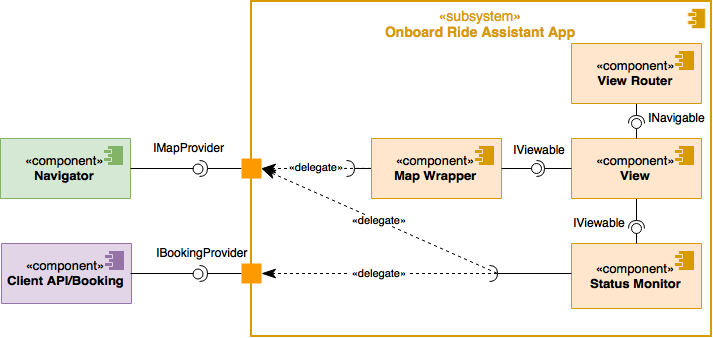
\includegraphics[scale=0.5]{{Figures/Component_Diagram/CarApp.png}}
\label{fig:CarApp}
\end{figure}
The Ride Assistant App is composed of:
\begin{itemize}
    \item\textbf{View}\newline
    It is a set of sub-components representing something the user can see and interact with; each sub-component renders the view relying on the view models provided by other components and translates user inputs to well-formed and sanitized requests sent through other components.
    For this application this set includes sub-components related to navigator, search input field, options and ride details.
    \item\textbf{View Router}\newline
    It is the component that implements and keep tracks of navigation paths across various views, providing for a given view model the right view component to be navigated that is able to present it to the user. It also implements backward navigation feature.
    \item\textbf{Map Wrapper}\newline
    It is the component that wraps the maps provided by the Navigator and makes it scrollable and zoomable, with the ability to overlay custom objects in defined position. It allows the application not to be coupled to a specific third-party navigation product.
    \item\textbf{Status Monitor}\newline
    It is the component that updates the ride details and the options available to the user: money saving alternative destination and Special Parking Areas listing.
\end{itemize}
and it interacts with:
\begin{itemize}
    \item\textbf{Navigator}\newline
    It is the third-party navigation software which provides navigation directions to the user, and translate the inserted addresses into precise coordinates. It also provides maps images to other components.
    \item\textbf{Client API/Booking}\newline
    \textit{See above.}
\end{itemize}
%Add \newpage here if necessary
\newpage

\subsection{Deployment view}
\begin{figure} [h!]
\centering
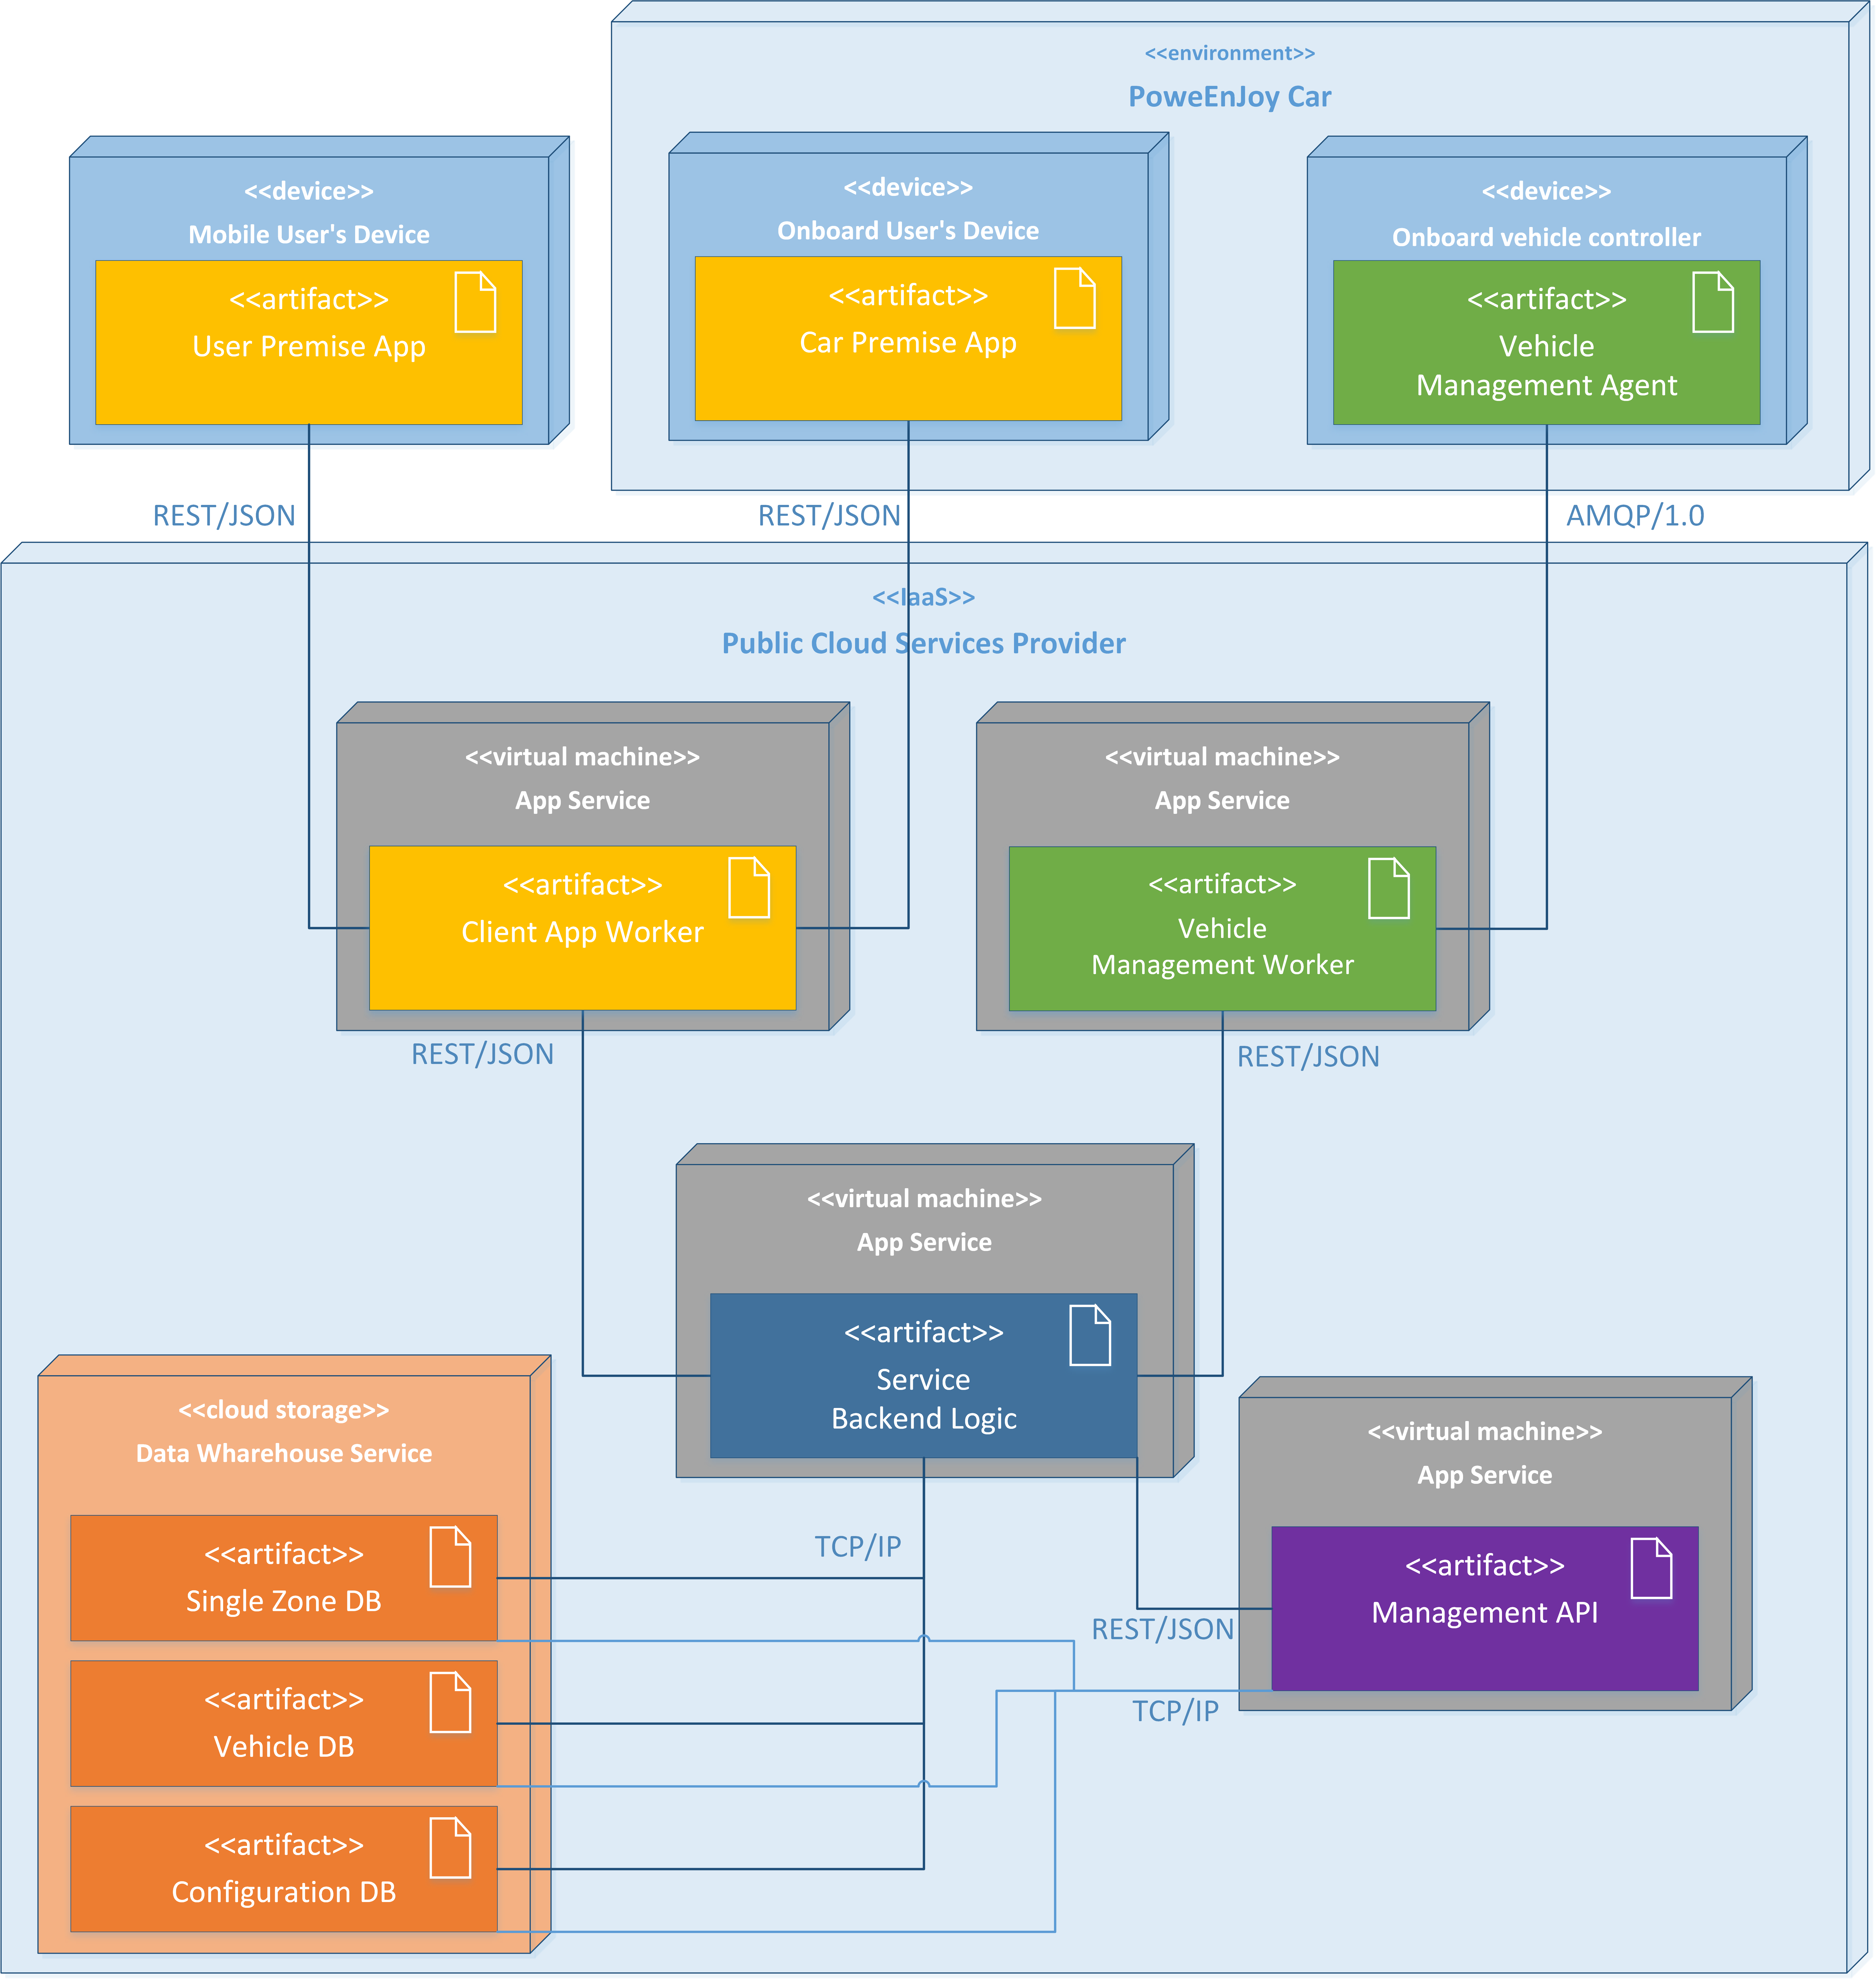
\includegraphics[scale=0.51]{{Figures/Deployment.png}}
\label{fig:Deployment}
\end{figure}
EXPLANATION TEXT
%Add \newpage here if necessary
\newpage


\subsection{Runtime view}

This section contains some Sequence Diagrams of the application.\\
In particular it shows what happens whenever:
\begin{itemize}
\item User send a request for unlock the Car;
\item User set ride destination and drive towards it; \newline
    the third diagram extends the second one and shows the Special Parking Area List and the Money Saving option features.
\end{itemize}

\newpage

\begin{landscape}
\begin{figure} [h!]
\centering
\includegraphics[scale=0.6]{{Figures/Sequence_Diagram/CarUnlock.png}}
\label{fig:UML Sequence Diagram: Car unlocking}
\caption{Car Unlocking}
\end{figure}
\end{landscape}

\newpage
\begin{landscape}
\begin{figure} [h!]
\centering
\includegraphics[scale=0.6]{{Figures/Sequence_Diagram/Ride.png}}
\label{fig:UML Sequence Diagram: Ride}
\caption{User's ride}
\end{figure}
\end{landscape}

\newpage

\begin{figure} [h!]
\centering
%scale=0.46
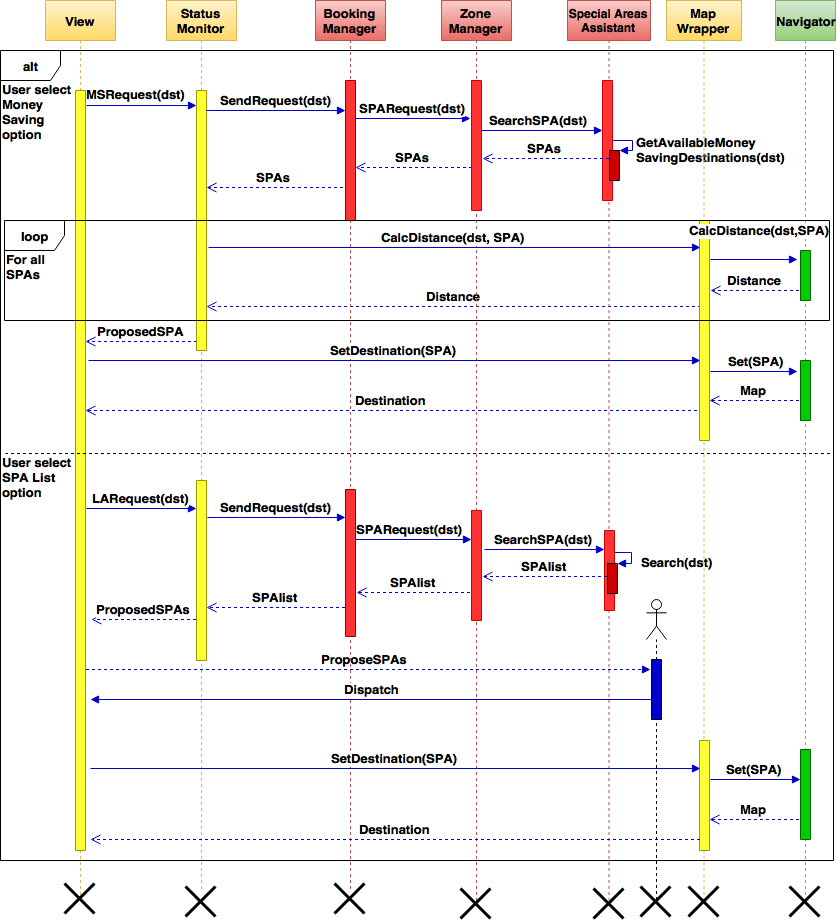
\includegraphics[scale=0.55]{{Figures/Sequence_Diagram/MS.png}}
\label{fig:UML Sequence Diagram: Money Saving and List Parking Area options}
\caption{Money Saving and List Parking Area options}
\end{figure}

\newpage

\subsection{Component interfaces}
In this section are defined the interfaces shown in the component view section. To make them easier to find they are listed in alphabetic order.
\begin{itemize}
    \item\textbf{TITLE}\newline
    EXPLANATION
    \item\textbf{TITLE}\newline
    EXPLANATION
    \item\textbf{TITLE}\newline
    EXPLANATION
    \item\textbf{TITLE}\newline
    EXPLANATION
    \item\textbf{TITLE}\newline
    EXPLANATION
    \item\textbf{TITLE}\newline
    EXPLANATION
    \item\textbf{TITLE}\newline
    EXPLANATION
    \item\textbf{TITLE}\newline
    EXPLANATION
    \item\textbf{TITLE}\newline
    EXPLANATION
    \item\textbf{TITLE}\newline
    EXPLANATION
    \item\textbf{TITLE}\newline
    EXPLANATION
    \item\textbf{TITLE}\newline
    EXPLANATION
\end{itemize}


\subsection{Selected architectural styles and patterns}
The solution described in this document strongly embrace modern cloud-oriented philosophy. We believe the PowerEnJoy service has those key characteristics that made the choice of a cloud architecture to fit very nicely our customer needings.
As most significant ones we would like to underline:
\begin{itemize}
    \item The PowerEnJoy system will be developed from scratch, this allows the adoption of most convenient and future-proof architectural designs.
    \item PowerEnJoy is a start-up company, cloud Infrastructures as a Service are well-known to minimize initial deployment costs and risks of capital in case of business failure.
    \item Car sharing services, at the moment are experiencing a significant growth in terms of user adoption, therefore exists a concrete chance that the architecture would be heavy loaded even on service launch date which will probably require huge resources deployment that will take relatively long time to be completed with on-premise infrastructures.
\end{itemize}
\subsubsection{Cloud Design Patterns}
Designing cloud-ready software solutions has an immediate positive side-effect: each single taken design decision must always keep that elasticity and abstraction level the environment itself is characterized by. This practically turns out into helping solution architects to avoid many kinds of bad and harmful decisions that often come from technological concerns. The PowerEnJoy software platform this document describes follows most common recommended guidelines and best practices about roles subdivision across virtual compute units, message queuing and processing, data replication and caching. For more detailed description of those concepts you can refer to the MSDN library article you find in the External References section (§\ref{external_ref}) of this document.

\subsubsection{Architectural Design Patterns}
The whole PowerEnJoy software platform consists of a distributed, multi-tier architecture with a presentation layer split into a common front-end proxy and two different remote mobile clients, a middle tier that implements the PowerEnJoy business logic, a data tier which splits into multiple datasources and an IoT tier which includes both remote embedded devices and incoming telemetry data proxy. Each remote mobile client adopt an MVC style pattern, but its actual interpretation varies across different frameworks supported by the target OSs.

\subsubsection{Communication Design Patterns}


\subsection{Other design decisions}
Following paragraphs refer to relevant design decisions not explicitly explained anywhere else in this document.\\

The SBL supports configurable timeout values for any event regarding a ride. This means no software upgrade is needed to change those values in case of requirements changes.\\

The SBL supports configurable discounts policies. This means that each required feature regarding discount applicability can be modified or updated in future without any software upgrade. Each discount policy is defined by a set of conditions to be satisfied at a specific point of a booking (on Car unlocking, on engine turn-off, on Car locking) and parameters that allow to modify the charged fare (percentage discount ratio, absolute discount amount).\\

As said in previous chapters, each zone served by PowerEnJoy can override any global setting from the shared configuration datasource.\\

The mobile clients are expected to evolve much more frequently with respect to other service components. Therefore sounds reasonable not to define further the MVC pattern variant technicalities, taking advantage of any platform specific framework which best integrates with the target at the time of development. These components are designed in such a way that the development of a brand-new version based on a completely different MVC framework should complete in short time and without generating issues to be addressed into other components of the solution, in the event of new target OSs release/update.\\ 

